\documentclass[a4paper]{article}
\usepackage[dutch]{babel}
\usepackage{amsmath}
\usepackage{amssymb}
\usepackage{graphicx}
\usepackage{mathtools}
\usepackage{float}
\usepackage{url}
\usepackage{algorithmicx}
\usepackage{algpseudocode}
\usepackage{algorithm}
\usepackage[T1]{fontenc}
\usepackage[framed,numbered]{matlab-prettifier}
\usepackage{subcaption}

\graphicspath{ {afbeeldingen/} }

\title{Numerieke Modellering en Benadering: Practicum 2}
\author{Ellen Anthonissen \and Marte Biesmans}
\date{donderdag 25 mei 2017}

\newcommand{\opgave}[1]{\subsection*{Opgave #1}}
\newcommand{\dx}{\Delta x}
\newcommand{\dy}{\Delta y}
\newcommand{\dz}{\Delta z}
\newcommand{\dt}{\Delta t}

\begin{document}
\maketitle

\section{Bivariate kleinste-kwadraten veeltermbenadering}

\opgave{1}
Onderstaande funtie berekent de co\"effici\"entenmatrix $C \in \mathbb{R}^({n+1) \times (m+1)}$, gegeven de vectoren $x \in \mathbb{R}^{M}$ en $y \in \mathbb{R}^{N}$ als 2D meetpunten, de matrix $F \in \mathbb{R}^{N \times M}$ met functie- of meetwaarden en de parameters $m,n \in \mathbb{N}$ die respectievelijk de graad in $x$ en $y$ van de benaderende veeltermen.
\lstinputlisting[
  style      = Matlab-editor,
  basicstyle = \mlttfamily,
]{kkb.m}

Er werd een kleine test op deze functie uitgevoerd. Hierbij is de input: $x = \begin{bmatrix}1&2&3\end{bmatrix}, y = \begin{bmatrix}1&2&3\end{bmatrix}, m = 3, n = 2$ en
$$F = \begin{bmatrix}1&2&1\\
2&3&2\\
1&2&1\end{bmatrix}.$$
De punten werden samen geplot met het benaderend oppervlak in figuur \ref{fig:oef11}.

\begin{figure}[htb]
    \centering
    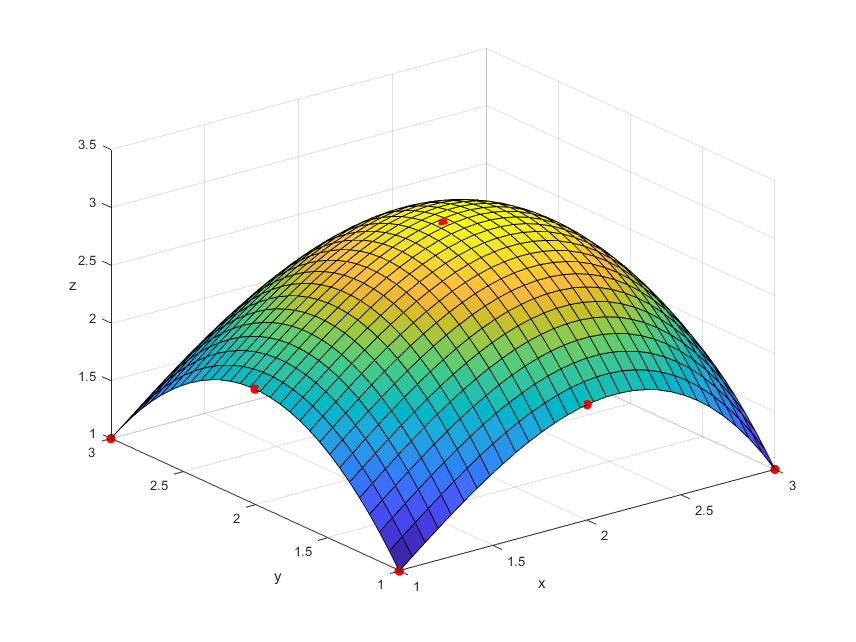
\includegraphics[width=0.7\textwidth]{oef11.png}
    \caption{test van het kkb algoritme}
    \label{fig:oef11}
\end{figure}

\opgave{2}
Voor de eerste dataset, gegenereerd door $f(x,y)=sin((2x-1)^2+2y)$ op elk punt van het rooster toe te passen, worden de veeltermbenadering van graad $7$ in $x$ en $y$ in het interval $[-1,1]\times [-1,1]$ en de exacte functiewaarden weergeven op de linkse grafiek van figuur ~\ref{fig:oef12}. 
Voor de tweede dataset, gegenereerd door $F = \texttt{membrane}(1,15)$ in MATLAB, worden de veeltermbenadering van graad $7$ in $x$ en $y$ en de exacte data weergeven op de rechtse grafiek van figuur~\ref{fig:oef12}.

\begin{figure}[H]
    \centering
    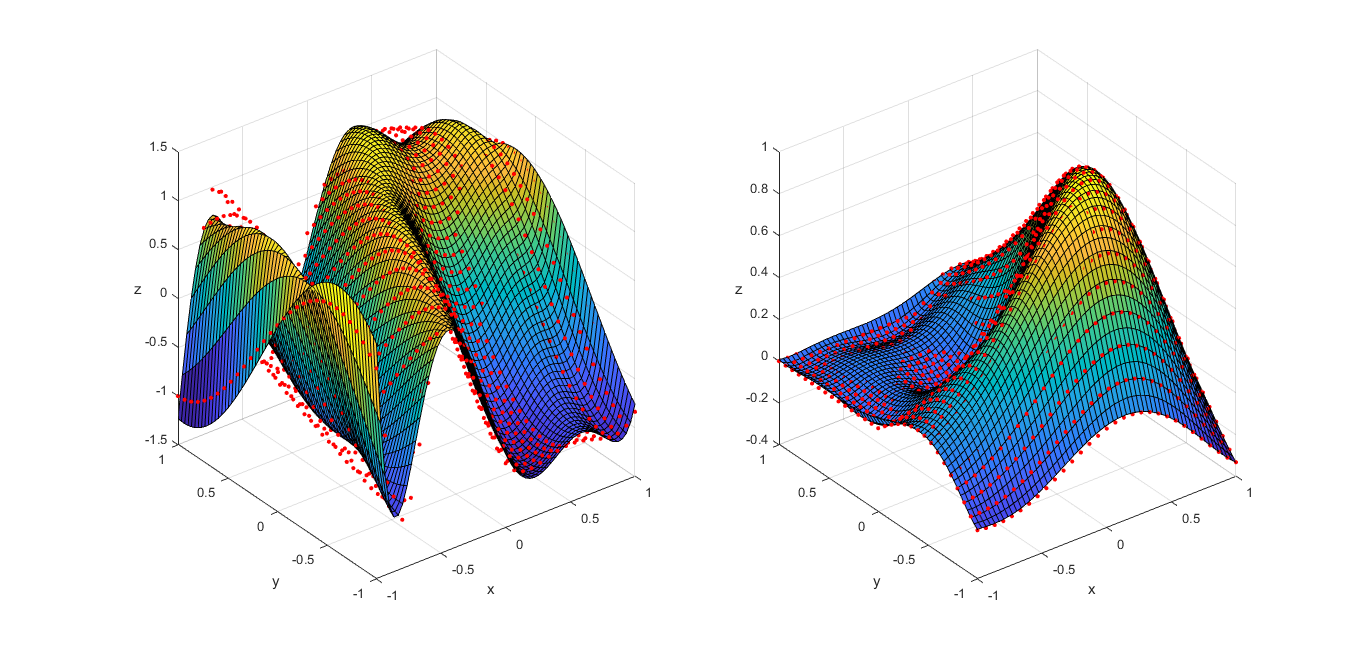
\includegraphics[width=1\textwidth]{oef12.png}
    \caption{veeltermbenadering van graad $7$ in $x$ en $y$ van de functie $f(x,y)=sin((2x-1)^2+2y)$ (links) en $F=\texttt{membrane}(1,15)$ (rechts)}
    \label{fig:oef12}
\end{figure}

\opgave{3}
De opeenvolgende waarden van de benaderingsfout $\lVert f-z_{mn} \rVert_2$ voor $m = n = 1,\dots,20$ voor beide datasets van opgave 2 worden weergegeven in figuur~\ref{fig:oef13}. We zien hier duidelijk dat voor de tweede dataset veeltermoppervlakken een geschikte benadering is. De eerste dataset heeft een slechte veeltermbenadering voor kleine $m,n$. Dat komt omdat de fuctie $f(x,y)=sin((2x-1)^2+2y)$ een zekere periodiciteit bevat en kan dus beter benaderd worden door middel van trigonometrische functies.

\begin{figure}[H]
    \centering
    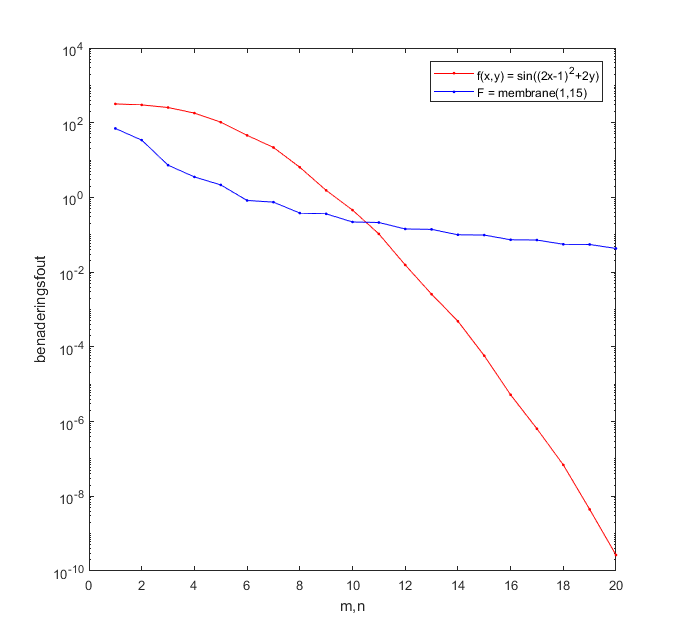
\includegraphics[width=0.5\textwidth]{oef13.png}
    \caption{benaderingsfout $\lVert f-z_{mn} \rVert_2^2$ van de veeltermbenadering van de functie $f(x,y)=sin((2x-1)^2+2y)$ en $F=\texttt{membrane}(1,15)$ in functie van de graad in $x$ en $y$}
    \label{fig:oef13}
\end{figure}

\opgave{4}
De veeltermbenadering van de functie van Runge $f(x,y)=\frac{1}{1+25(x^2+y^2)}$ gebruik makend van twee verschillende roosters wordt getoond in figuur~\ref{fig:oef14resultaat}.
Zowel een rooster met equidistante punten (links) als een rooster met niet-equidistante punten (rechts) werd gebruikt ter vergelijking.

\begin{figure}[H]
    \centering
    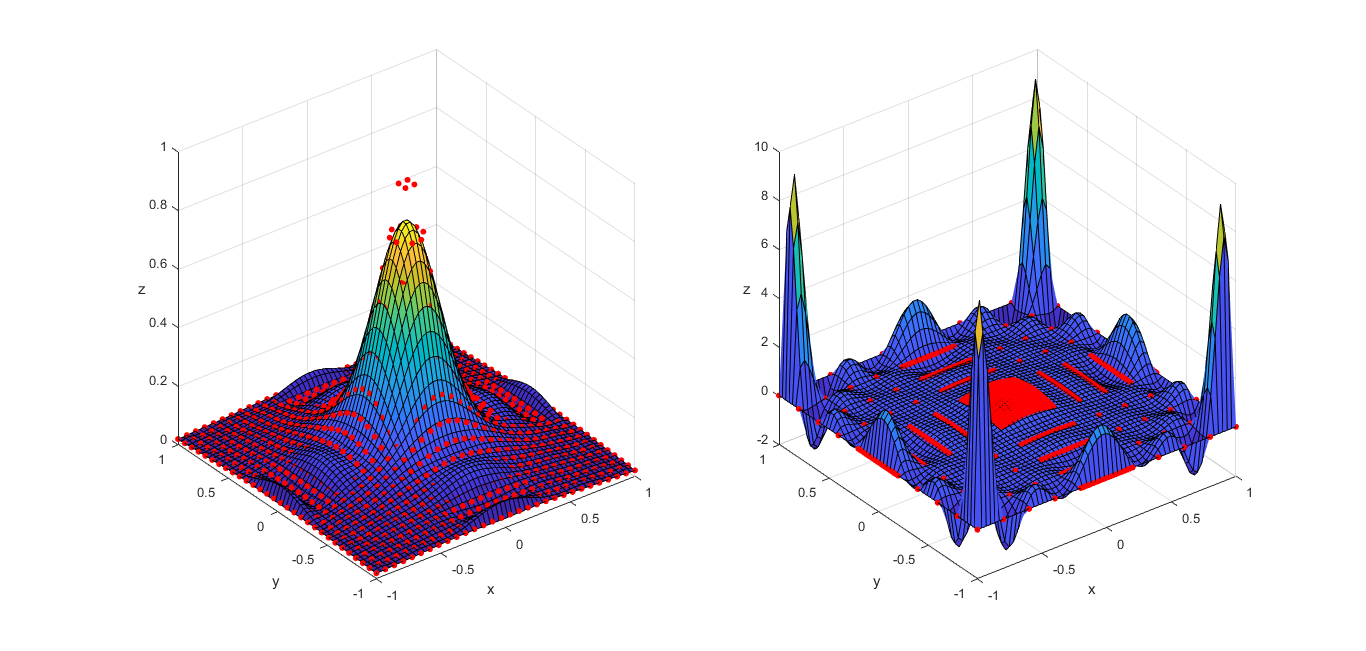
\includegraphics[width=1\textwidth]{oef1410.png}
    \caption{veeltermbenadering van graad $10$ in $x$ en $y$ van de functie van Runge $f(x,y)=\frac{1}{1+25(x^2+y^2)}$ gebruik makend van equidistante roosterpunten (links) en niet-equidistante roosterpunten (rechts)}
    \label{fig:oef14resultaat}
\end{figure}

Het is hier duidelijk dat het rooster dat gebruik maakt van een equidistante verdeling te verkiezen is. Dit komt doordat bij de niet-equidistante verdeling er weinig aandacht gaat naar de randen van het 2D interval. Bij het verhogen van de graad van de veeltermbenadering gaan er zich namelijk grote schommelingen voordoen aan de rand van het interval. Dit zorgt voor een zeer grote maximale fout bij hogere machten, die voorkomt in de hoekpunten (zie figuur~\ref{fig:oef14} rechts). We zien ook dat de benaderingsfout $\lVert f-z_{mn} \rVert_2^2$ (figuur~\ref{fig:oef14}) en de maximale afwijking (figuur~\ref{fig:oef14}) voor een niet-equidistante verdeling toch beperkt blijft voor $m,n \leq 15$, terwijl het benaderende veeltermoppervlak toch niet zo goed is. De fout bij de roosterpunten blijft inderdaad beperkt, maar de fout buiten de roosterpunten is daarentegen wel groot. De niet-equidistante verdeling van roosterpunten geeft wel een goede benadering van de functie van Runge rond de oorsprong.

\begin{figure}[H]
    \centering
    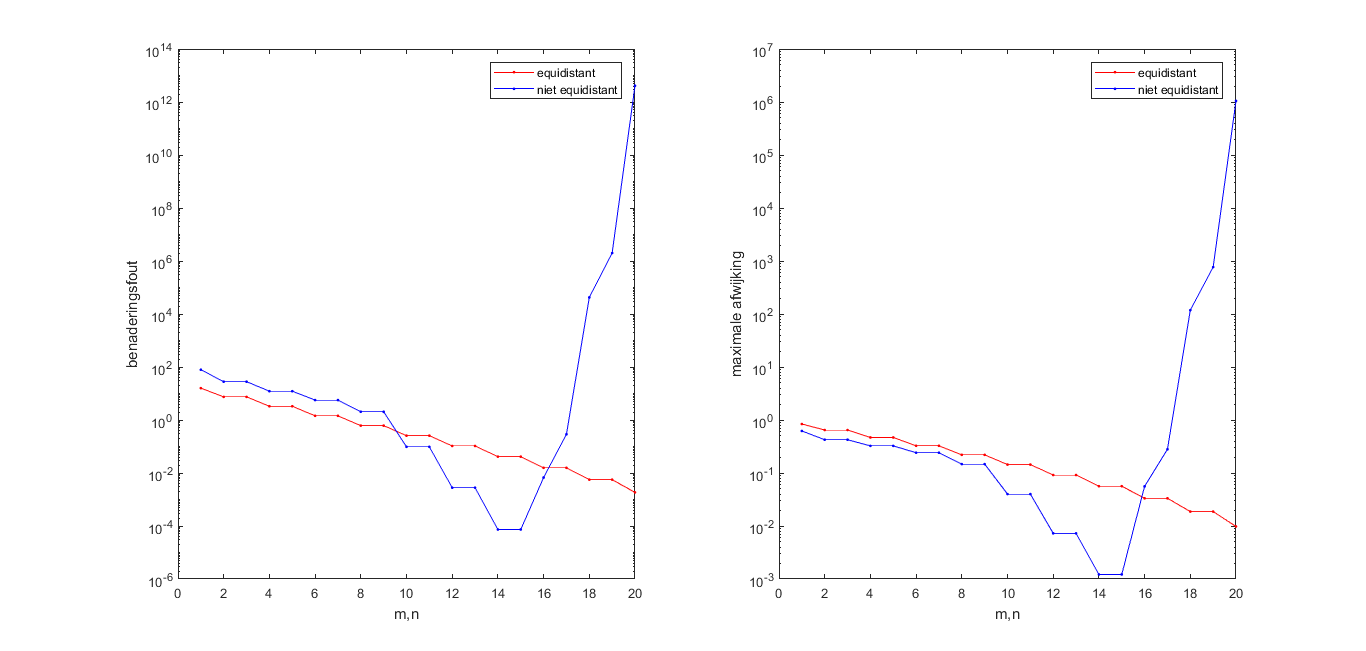
\includegraphics[width=1\textwidth]{oef14.png}
    \caption{benaderingsfout $\lVert f-z_{mn} \rVert_2^2$ (links) en de maximale afwijking (rechts) van de veeltermbenadering van de functie van Runge $f(x,y)=\frac{1}{1+25(x^2+y^2)}$ in functie van de graad in $x$ en $y$}
    \label{fig:oef14}
\end{figure}



\opgave{5}
De veeltermbenadering van de Etna van graad $25$ in $x$ en $y$ wordt getoond in figuur~\ref{fig:oef15}. Voor $M$ en $N$ werd het aantal pixels gekozen in de x en y richting respectievelijk gekozen.

\begin{figure}[H]
    \centering
    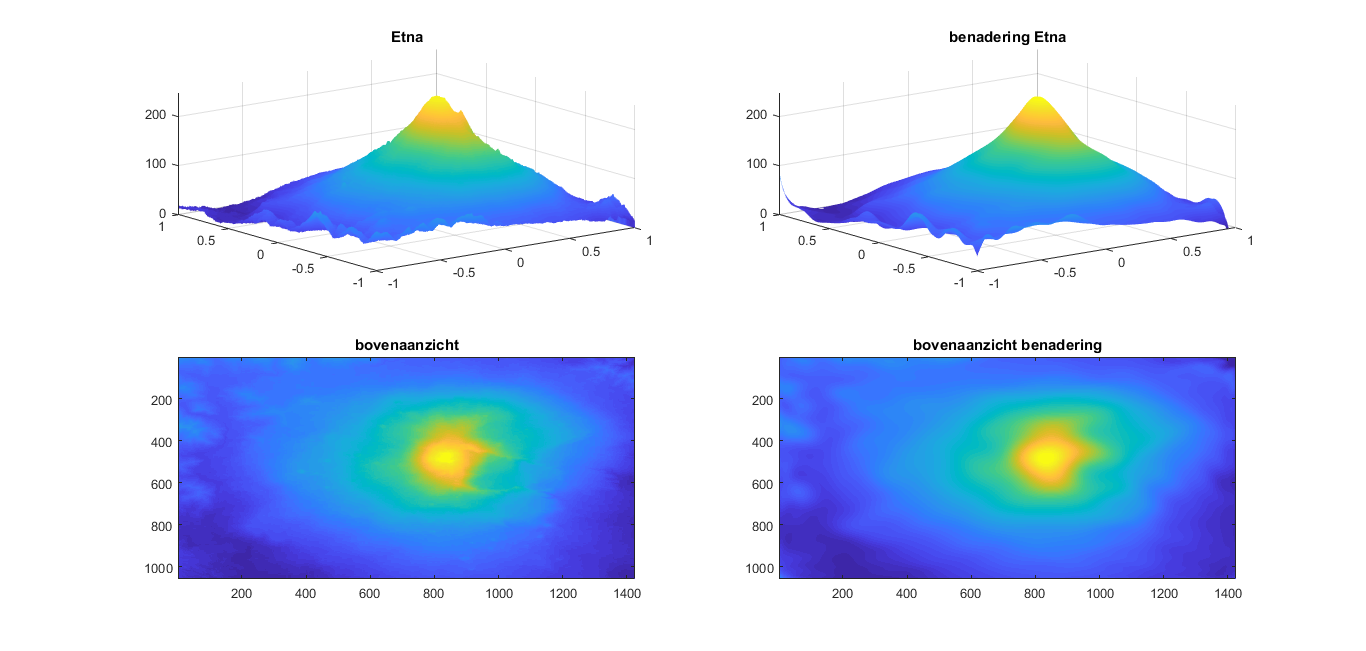
\includegraphics[width=0.8\textwidth]{oef15.png}
    \caption{3D-weergave en bovenaanzicht van de Etna (links) en van de benadering (rechts)}
    \label{fig:oef15}
\end{figure}

\section{Interpolerente splinefuncties en -curven}

\opgave{1}
plaats code hier\\
Om de correctheid van de implementatie te testen hebben we de functie sin(x) benaderd op het interval [-2,2] met equidistante punten. Hierbij gebruikten we 4 abscissen en 11 evaluatiepunten. Door dit zowel op papier als in matlab uit te rekenen kunnen stap per stap de waarden voor A, b, S, $c_1$, $c_2$ en y gecontroleerd worden.

\opgave{2}
We gebruiken bovenstaande code om $sin(x)$ en $\frac{1}{1+7x^2}$ te benaderen op het interval [-2,2] met een equidistante set van 10 abscissen voor $sin(x)$ en 9 abscissen voor de tweede functie. We vergelijken dit ook met een veelterminterpolant door deze punten. Voor deze veelterm gebruiken we de graad N-1, met N het aantal abscissen. Het eerste resultaat is te vinden in figuur \ref{fig:sinequi}, het tweede resultaat in figuur \ref{fig:ratequi}. We geven steeds een plot van de functiewaarden en van de absolute waarde van het residu weer. In de abscissen gaat de fout tot op machineprecisie. Dit is niet zichtbaar in de figuur aangezien de figuur getekend wordt op basis van een aantal evaluatiepunten.

Voor de sinusfunctie presteert de veeltermbenadering beter. Dit is te verklaren doordat de veeltermbenadering de afgebroken reeksontwikkeling van de sinus vormt.

De functie $\frac{1}{1+7x^2}$ is een klassiek voorbeeld van een functie die slecht te banderen is met een interpolerende veelterm door equidistante punten. Dit is duidelijk te zien in de plot. De splinevoorstelling presteert hier een stuk beter.

\begin{figure}[H]
\centering
\begin{subfigure}{.5\textwidth}
  \centering
  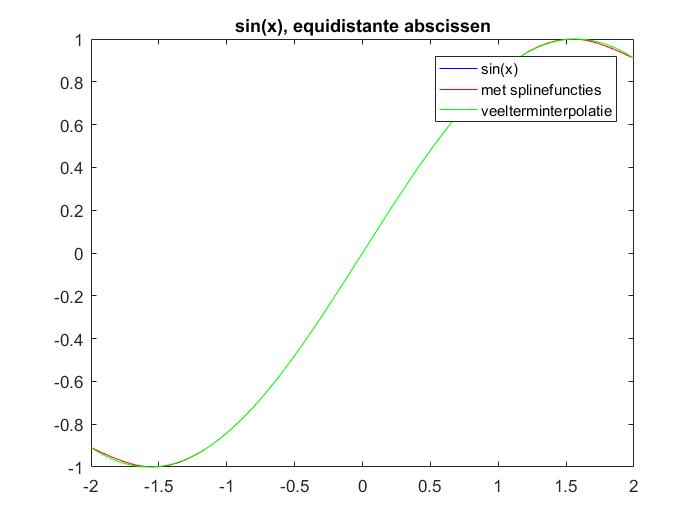
\includegraphics[width=\linewidth]{afbeeldingen/sin_equi.jpg}
  \caption{functiewaarden}
\end{subfigure}%
\begin{subfigure}{.5\textwidth}
  \centering
  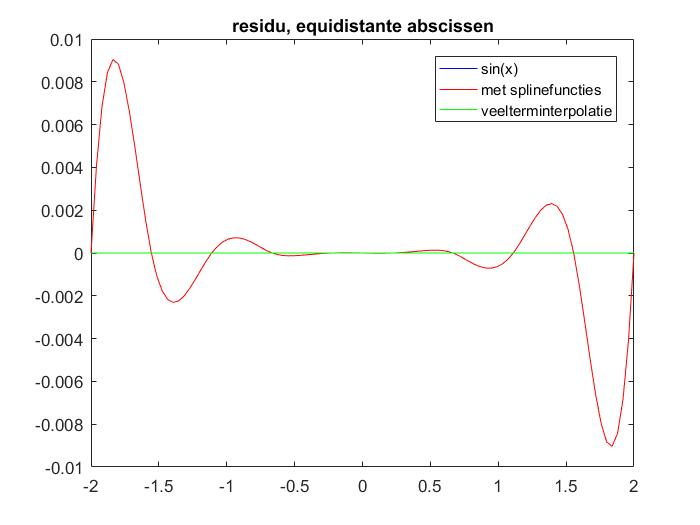
\includegraphics[width=\linewidth]{afbeeldingen/sin_equi_res.jpg}
  \caption{residu}
\end{subfigure}
\caption{interpolant door 10 equidistante absciswaarden van $sin(x)$}
\label{fig:sinequi}
\end{figure}

\begin{figure}[H]
\centering
\begin{subfigure}{.5\textwidth}
  \centering
  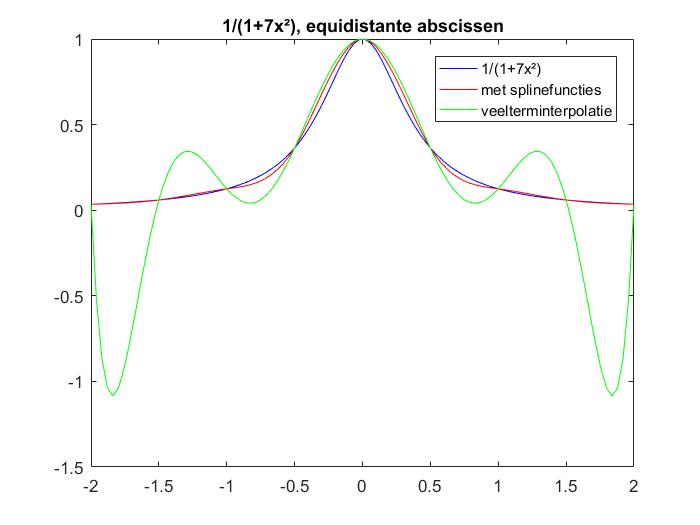
\includegraphics[width=\linewidth]{afbeeldingen/rat_equi.jpg}
  \caption{functiewaarden}
\end{subfigure}%
\begin{subfigure}{.5\textwidth}
  \centering
  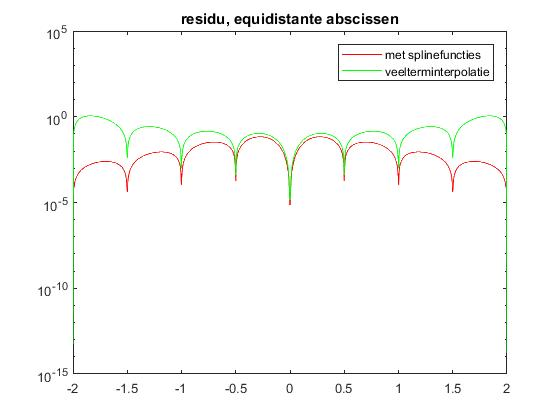
\includegraphics[width=\linewidth]{afbeeldingen/rat_equi_res.jpg}
  \caption{residu}
\end{subfigure}
\caption{interpolant door 9 equidistante absciswaarden van $\frac{1}{1+7x^2}$}
\label{fig:ratequi}
\end{figure}

\opgave{3}
Nu doen we hetzelfde, maar in plaats van equidistante abscissen gebruiken we nu Chebyshev-punten. Het  resultaat voor $sin(x)$ is te vinden in figuur \ref{fig:sincheb}, het resultaat voor $\frac{1}{1+7x^2}$ in figuur \ref{fig:ratcheb}. We geven ook hier steeds een plot van de functiewaarden en van het residu weer.
\\
Het gebruik van Chebyshev-punten is een duidelijke verbetering, vooral aan de rand van het interval. 
\\
TODO verdere uitleg over verschil veelterm vs. spline

\begin{figure}
\centering
\begin{subfigure}{.5\textwidth}
  \centering
  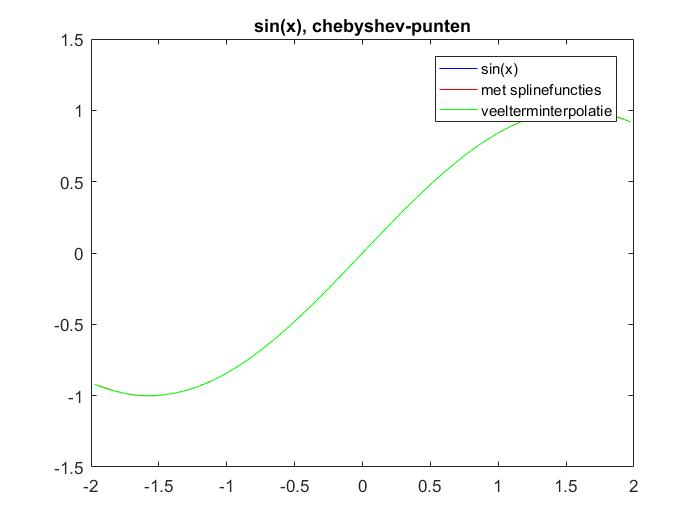
\includegraphics[width=\linewidth]{afbeeldingen/sin_cheb.jpg}
  \caption{functiewaarden}
\end{subfigure}%
\begin{subfigure}{.5\textwidth}
  \centering
  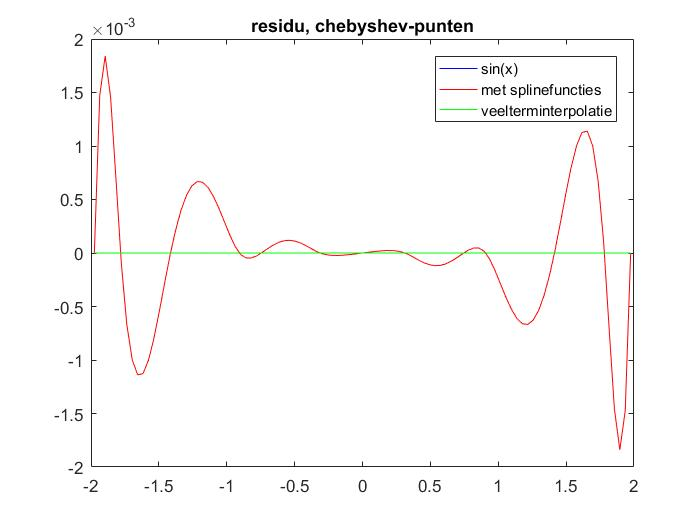
\includegraphics[width=\linewidth]{afbeeldingen/sin_cheb_res.jpg}
  \caption{residu}
\end{subfigure}
\caption{interpolant door 10 Chebyshev-punten van $sin(x)$}
\label{fig:sincheb}
\end{figure}

\begin{figure}
\centering
\begin{subfigure}{.5\textwidth}
  \centering
  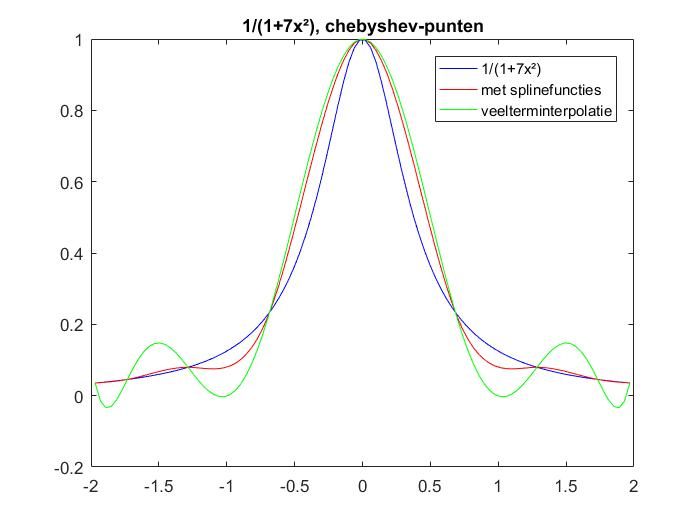
\includegraphics[width=\linewidth]{afbeeldingen/rat_cheb.jpg}
  \caption{functiewaarden}
\end{subfigure}%
\begin{subfigure}{.5\textwidth}
  \centering
  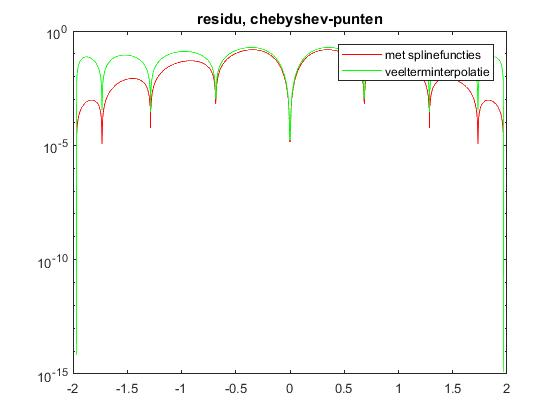
\includegraphics[width=\linewidth]{afbeeldingen/rat_cheb_res.jpg}
  \caption{residu}
\end{subfigure}
\caption{interpolant door 9 Chebychev-punten van  $\frac{1}{1+7x^2}$}
\label{fig:ratcheb}
\end{figure}

\opgave{4}
We kozen als griekse letters de letters delta en phi aangezien deze geen scherpe knikken bevatten. Het resultaat is te zien in figuur \ref{fig:griekse_letters}. De aangeduide punten zijn de inputgegevens, de rode lijn is de berekende curve.

\begin{figure}[H]
\centering
\begin{subfigure}{.5\textwidth}
  \centering
  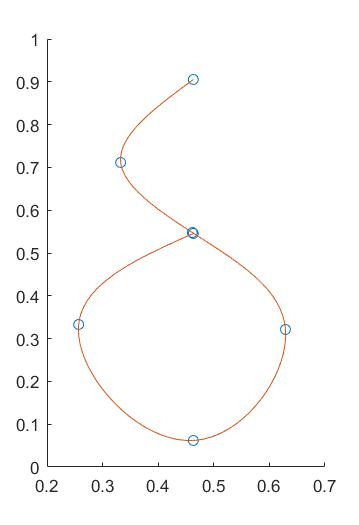
\includegraphics[width=.4\linewidth]{afbeeldingen/delta_result.jpg}
  \caption{delta}
\end{subfigure}%
\begin{subfigure}{.5\textwidth}
  \centering
  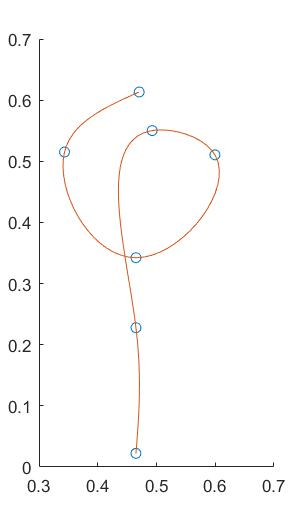
\includegraphics[width=.4\linewidth]{afbeeldingen/phi_result.jpg}
  \caption{phi}
\end{subfigure}
\caption{griekse letters benaderd door interpolerende, kubische splinecurven}
\label{fig:griekse_letters}
\end{figure}

In figuur \ref{fig:lalinea} zie je op dezelfde manier de splinevoorstelling van het mannetje van La Linea. Ook hier ziet men duidelijk dat knikken niet worden weergegeven. Dit is logisch aangezien dit een ander probleem is dan het opstellen van een natuurlijke, interpolerende, kubische splinecurve. Er zouden immers andere voorwaarden opgelegd worden aan de verschillende afgeleiden.

\begin{figure}[H]
    \centering
    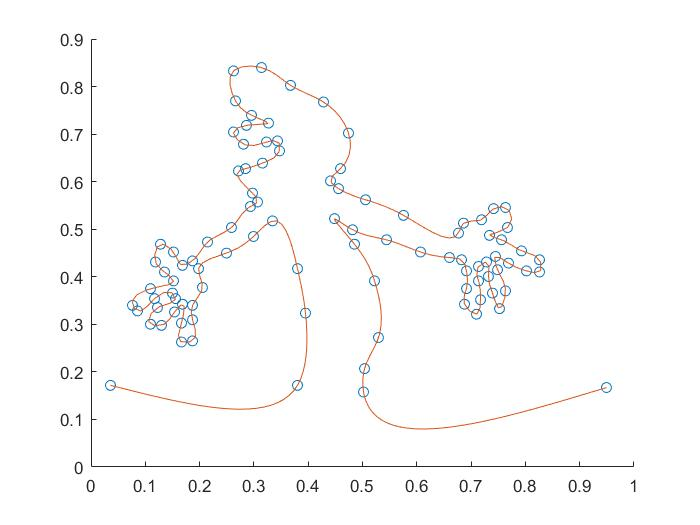
\includegraphics[width=0.7\textwidth]{lalinea_result.jpg}
    \caption{splinevoorstelling van het mannetje van La Linea}
    \label{fig:lalinea}
\end{figure}

\end{document}